\documentclass[11pt,a4paper]{article}
\usepackage[utf8]{inputenc}
\usepackage{amsmath,amsfonts,amssymb}
\usepackage{graphicx}
\usepackage{geometry}
\geometry{margin=1in}
\usepackage{booktabs}
\usepackage{hyperref}
\usepackage{float}
\usepackage{xcolor}

\definecolor{darkbg}{HTML}{0d121f}
\definecolor{lighttext}{HTML}{e2e8f0}
\definecolor{primary}{HTML}{8b5cf6}
\definecolor{secondary}{HTML}{0dd5c5}
\definecolor{accent}{HTML}{10b981}

\pagecolor{darkbg}
\color{lighttext}

\hypersetup{
    colorlinks=true,
    linkcolor=secondary,
    urlcolor=secondary,
    citecolor=accent
}

\title{\textbf{EE3621: Digital Signal Processing} \\ \Large Student Lecture Notes — Lecture 21 \\ \large Linear Phase FIR Filters, Characteristics, Zeros \& Moving Average Filters}
\author{III B.Tech EEE — Core Exam Preparation Guide}
\date{}

\begin{document}

\maketitle

\noindent\rule{\textwidth}{0.5pt}

\section{Core Definitions \& Linear Phase Conditions}

\subsection{Distortionless Transmission \& Phase Delay vs. Group Delay}
An LTI filter transmits an input signal without waveform distortion if all frequency components experience:
\begin{enumerate}
    \item A constant gain: $|H(e^{j\omega})| = A_0$
    \item A strictly constant time delay: $\tau_g = \alpha$
\end{enumerate}
\begin{itemize}
    \item \textbf{Phase Delay:} The time delay experienced by each individual sinusoidal carrier:
    \begin{equation}
    \tau_p(\omega) = -\frac{\theta(\omega)}{\omega}
    \end{equation}
    \item \textbf{Group Delay:} The time delay experienced by the signal's modulation envelope:
    \begin{equation}
    \tau_g(\omega) = -\frac{d\theta(\omega)}{d\omega}
    \end{equation}
\end{itemize}
\textbf{The Linear Phase Criterion:} If $\theta(\omega) = -\alpha \omega$, then $\tau_p(\omega) = \tau_g(\omega) = \alpha = \text{constant}$. This eliminates \textbf{phase distortion} and \textbf{envelope dispersion}.

\subsection{Time-Domain Conditions for Linear Phase}
For a causal FIR filter of length $N$ (coefficients $h[0], h[1], \dots, h[N-1]$):
\begin{itemize}
    \item \textbf{Strict Linear Phase} ($\theta(\omega) = -\alpha \omega$): Requires \textbf{even symmetry}:
    \begin{equation}
    \mathbf{h[n] = h[N-1-n]}, \quad \alpha = \frac{N-1}{2}
    \end{equation}
    \item \textbf{Generalized Linear Phase} ($\theta(\omega) = \beta - \alpha \omega$, where $\beta = \pm \pi/2$): Requires \textbf{odd antisymmetry}:
    \begin{equation}
    \mathbf{h[n] = -h[N-1-n]}, \quad \alpha = \frac{N-1}{2}
    \end{equation}
\end{itemize}

\noindent\rule{\textwidth}{0.5pt}

\section{The 4 Linear-Phase FIR Filter Types (Master Reference)}

Every linear-phase FIR filter belongs to one of four distinct classes based on coefficient symmetry and length parity:

\begin{table}[H]
\centering
\caption{Classification and Filter Suitability of Linear-Phase FIR Filters}
\label{tab:fir_types}
\vspace{2mm}
\resizebox{\textwidth}{!}{
\begin{tabular}{cccccc}
\toprule
\textbf{Type} & \textbf{Symmetry} & \textbf{Length $N$} & \textbf{Phase $\theta(\omega)$} & \textbf{Mandatory Zeros} & \textbf{Filter Suitability} \\
\midrule
\textbf{Type 1} & Symmetric ($h[n]=h[N-1-n]$) & \textbf{Odd} ($M$ even) & $-\alpha\omega$ & None & \textbf{Universal: LPF, HPF, BPF, BSF} \\
\textbf{Type 2} & Symmetric ($h[n]=h[N-1-n]$) & \textbf{Even} ($M$ odd) & $-\alpha\omega$ & $\mathbf{\omega = \pi}$ ($z = -1$) & \textbf{LPF, BPF only} (Never HPF/BSF!) \\
\textbf{Type 3} & Antisymmetric ($h[n]=-h[N-1-n]$) & \textbf{Odd} ($M$ even) & $\frac{\pi}{2}-\alpha\omega$ & $\mathbf{\omega = 0, \pi}$ ($z = \pm 1$) & \textbf{BPF only} (Never LPF/HPF/BSF) \\
\textbf{Type 4} & Antisymmetric ($h[n]=-h[N-1-n]$) & \textbf{Even} ($M$ odd) & $\frac{\pi}{2}-\alpha\omega$ & $\mathbf{\omega = 0}$ ($z = 1$) & \textbf{HPF, BPF, Differentiator} \\
\bottomrule
\end{tabular}
}
\end{table}

\noindent\textbf{Critical Exam Insights:}
\begin{itemize}
    \item \textbf{Why Type 2 cannot be Highpass:} At $\omega = \pi$, $e^{j\pi(n - \alpha)} = \cos(\pi(n - \alpha))$. For $N$ even, $\alpha = (N-1)/2$ is a half-integer, making $\cos(\pi(n - \alpha)) = 0$. Hence, $\mathbf{H(e^{j\pi}) \equiv 0}$ unconditionally!
    \item \textbf{Why Antisymmetric Filters (Types 3 \& 4) have zero at $\omega = 0$:} Since $h[n] = -h[N-1-n]$, setting $\omega = 0$ gives $H(e^{j0}) = \sum h[n] = 0$. They block DC completely.
\end{itemize}

\noindent\rule{\textwidth}{0.5pt}

\section{Location of Zeros in the Complex Z-Plane}

Linear phase imposes reciprocal symmetry on the system function:
\begin{equation}
H(z) = \pm z^{-(N-1)} H(z^{-1})
\end{equation}
Consequently, if $z_0 = r e^{j\phi}$ is a zero of $H(z)$, its reciprocal $1/z_0 = \frac{1}{r} e^{-j\phi}$ must also be a zero. For real impulse responses, complex zeros must also occur in conjugate pairs.

\begin{figure}[H]
\centering
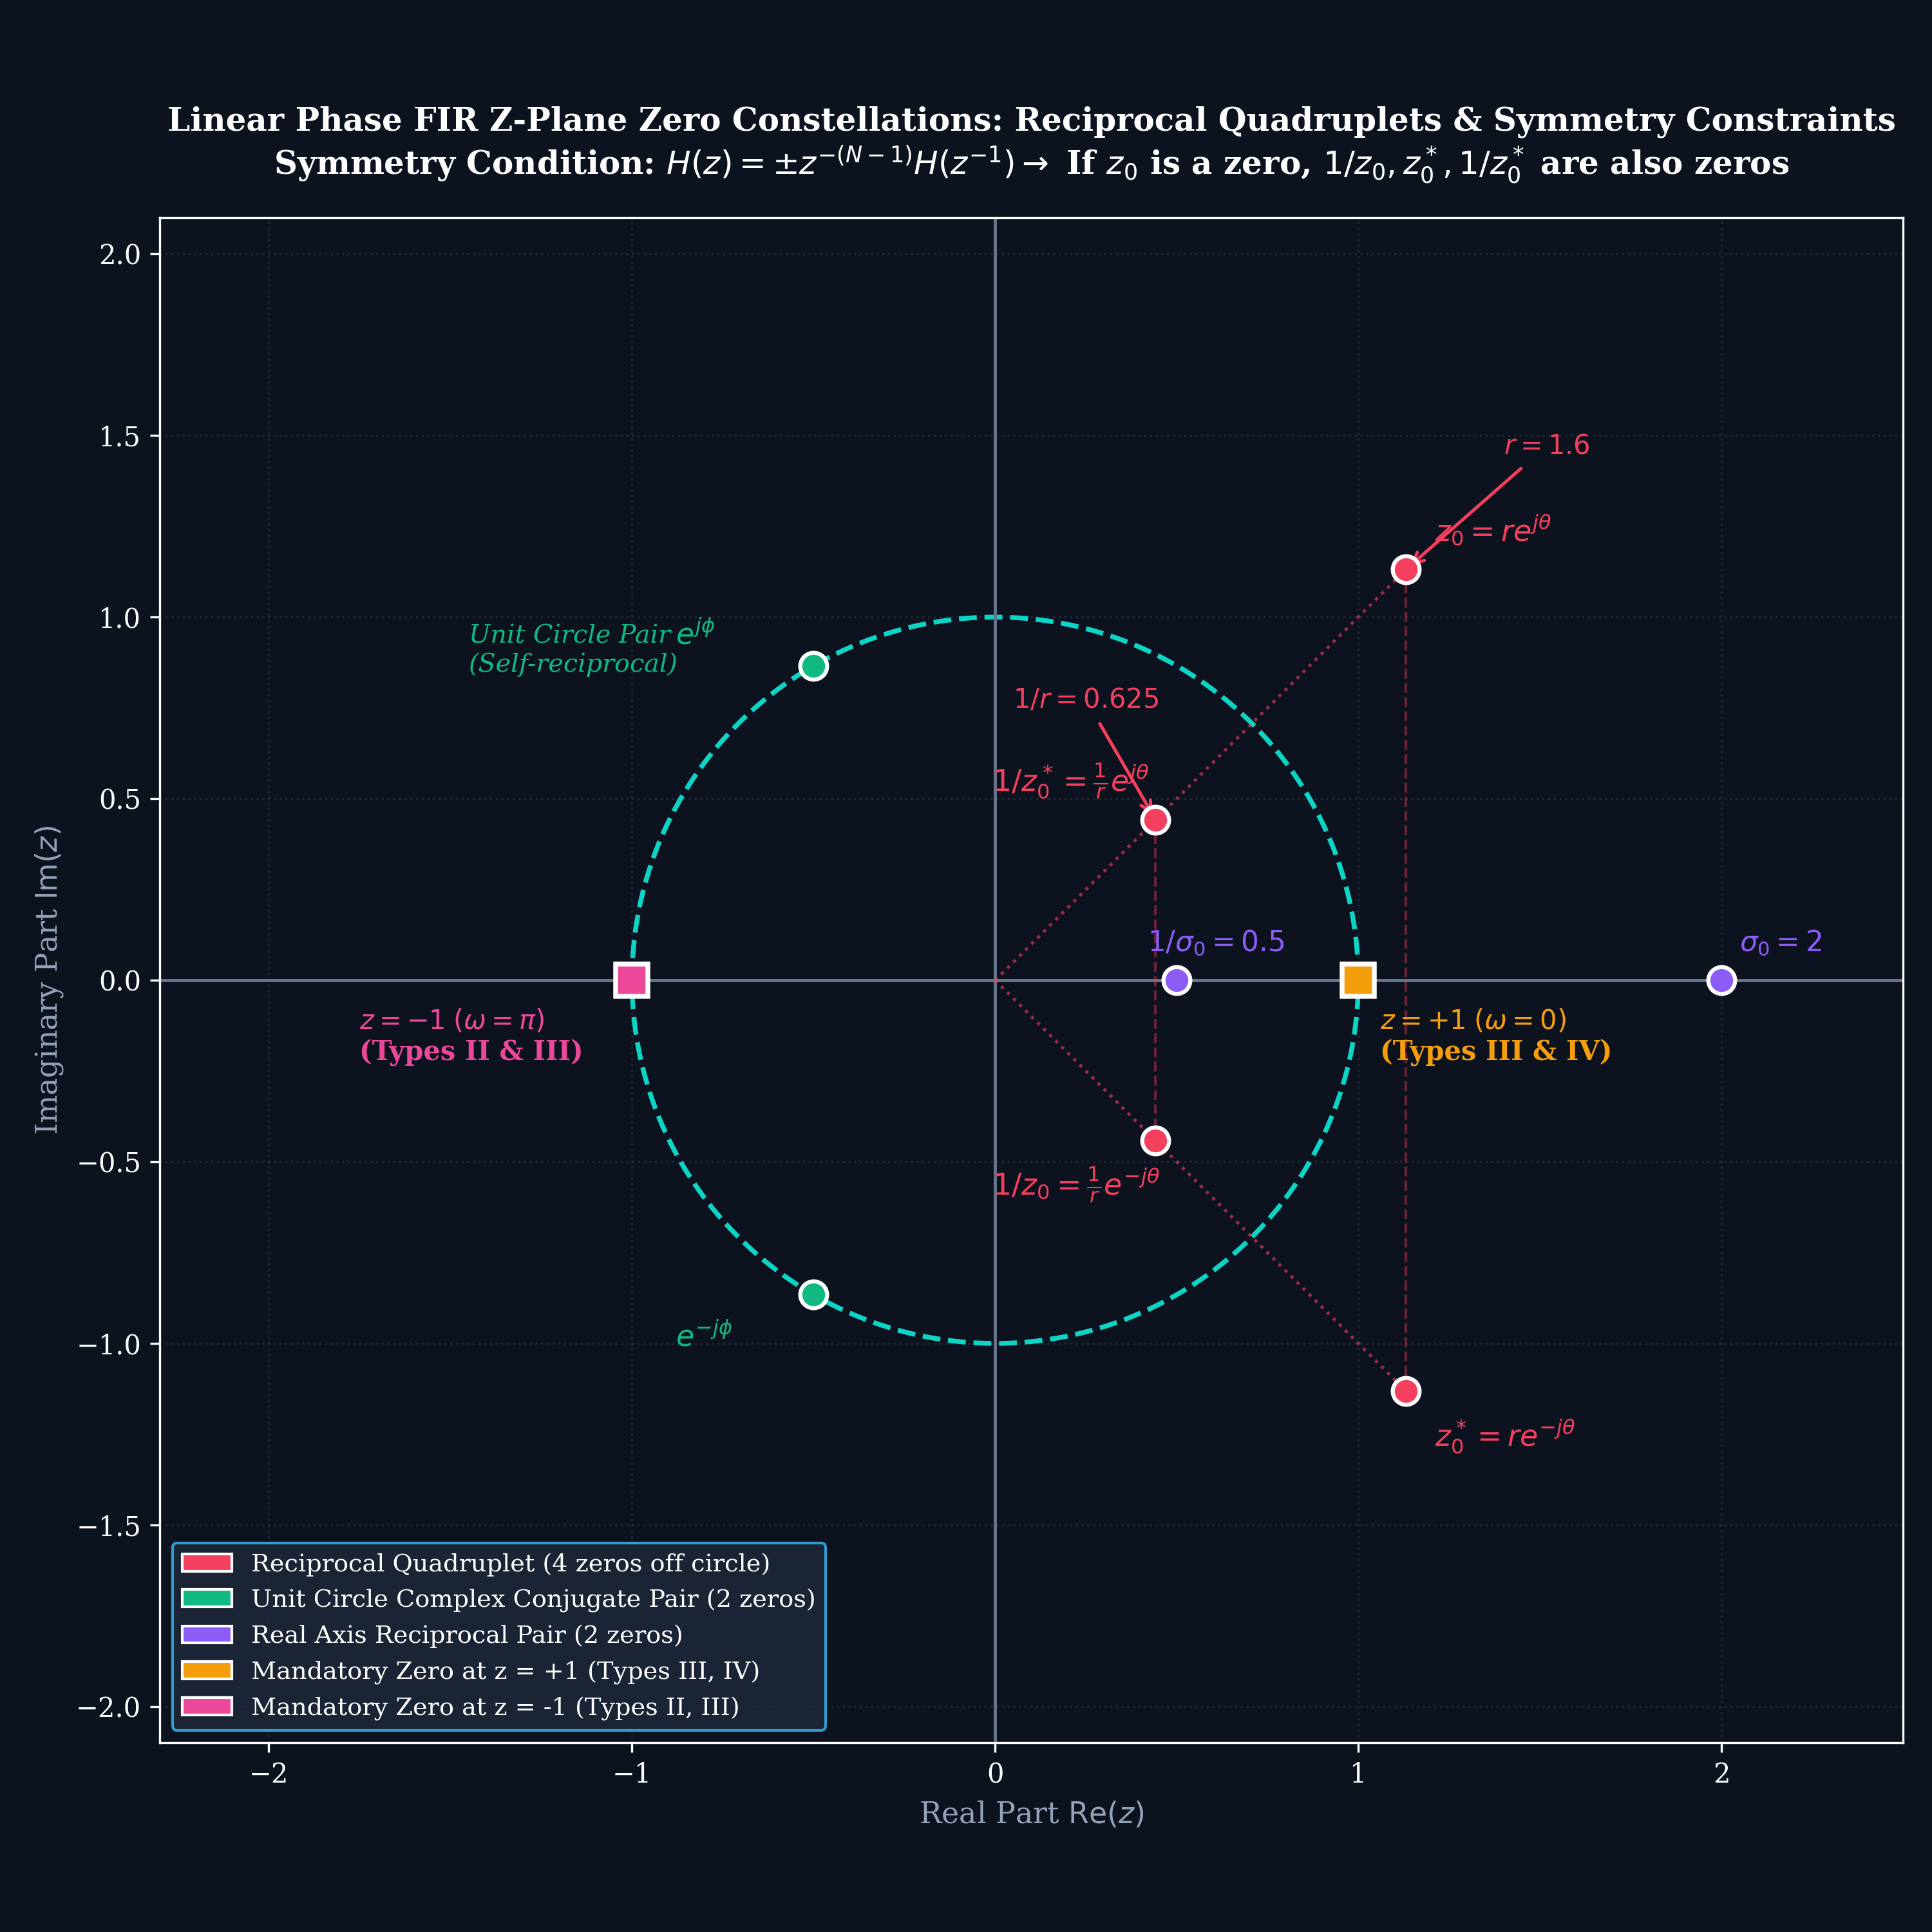
\includegraphics[width=0.7\textwidth]{images/fir_zero_locations_zplane.png}
\caption{Zero constellations for linear-phase FIR systems: complex quadruplets off the unit circle, pairs on the unit circle ($|z|=1$), and mandatory boundary zeros at $z = \pm 1$.}
\label{fig:zeros_zplane}
\end{figure}

\begin{itemize}
    \item \textbf{Complex zero off the unit circle ($|z| \ne 1$):} Appears as a \textbf{reciprocal conjugate quadruplet of 4 zeros}:
    \begin{equation}
    \left\{ r e^{j\phi}, \quad r e^{-j\phi}, \quad \frac{1}{r} e^{j\phi}, \quad \frac{1}{r} e^{-j\phi} \right\}
    \end{equation}
    \item \textbf{Complex zero on the unit circle ($|z| = 1$):} Since $1/e^{j\phi} = e^{-j\phi}$, the zero is its own reciprocal. It occurs as a \textbf{conjugate pair of 2 zeros}:
    \begin{equation}
    \left\{ e^{j\phi}, \quad e^{-j\phi} \right\}
    \end{equation}
    These zeros create sharp transmission nulls in the filter's stopband.
    \item \textbf{Real zero off the unit circle:} Occurs as a \textbf{reciprocal pair of 2 zeros}: $\{\sigma, \; 1/\sigma\}$.
    \item \textbf{Real zero on the unit circle:} A single zero at $z = 1$ ($\omega = 0$) or $z = -1$ ($\omega = \pi$).
\end{itemize}

\noindent\rule{\textwidth}{0.5pt}

\section{Moving Average (MA) Filters}

\subsection{Basic Equations}
An $M$-point Moving Average filter is defined by:
\begin{equation}
y[n] = \frac{1}{M}\sum_{k=0}^{M-1} x[n-k] \iff h[n] = \frac{1}{M}, \quad 0 \le n \le M-1
\end{equation}
\begin{itemize}
    \item \textbf{Symmetry:} $h[n] = h[M-1-n] = \frac{1}{M}$ $\implies$ \textbf{Always Linear Phase} with group delay $\tau = \frac{M-1}{2}$.
    \item \textbf{Frequency Response:}
    \begin{equation}
    H(e^{j\omega}) = \left[ \frac{\sin(M\omega/2)}{M\sin(\omega/2)} \right] e^{-j \left(\frac{M-1}{2}\right)\omega}
    \end{equation}
    \item \textbf{Zeros in Z-Domain:} $H(z) = \frac{1}{M} \frac{1 - z^{-M}}{1 - z^{-1}}$. The numerator has zeros at the $M$ roots of unity $e^{j 2\pi k / M}$. The zero at $k=0$ ($z=1$) is cancelled by the denominator pole at $z=1$.
    \item Exactly $M-1$ zeros lie on the unit circle: $\mathbf{z_k = e^{j \frac{2\pi k}{M}}}$ for $k = 1, 2, \dots, M-1$, producing transmission notches at harmonic frequencies.
\end{itemize}

\noindent\rule{\textwidth}{0.5pt}

\section{Standard Solved Exam Example}

\textbf{Problem:} An FIR filter has the impulse response:
\begin{equation}
h[n] = \{1, \; 2, \; 3, \; 2, \; 1\}, \quad \text{for } n = 0, 1, 2, 3, 4
\end{equation}
\begin{enumerate}
    \item Verify linear phase and determine the group delay $\tau_g$.
    \item Identify the filter type (Type 1 to 4) and its filter suitability.
    \item Find the amplitude function $A(\omega)$ and evaluate the DC gain $H(e^{j0})$.
    \item Find all zeros of $H(z)$ and sketch their constellation.
\end{enumerate}

\vspace{1mm}
\noindent\textbf{Solution:}

\noindent\textbf{Step 1: Symmetry and Group Delay}
Length $N = 5$ (Odd). Center of symmetry: $\alpha = \frac{N-1}{2} = \frac{5-1}{2} = 2$.
Checking symmetry: $h[0] = h[4] = 1$, $h[1] = h[3] = 2$, $h[2] = 3$.
Since $h[n] = h[4-n]$, the filter has \textbf{even symmetry} with constant group delay:
\begin{equation}
\mathbf{\tau_g = \alpha = 2 \text{ samples}}
\end{equation}

\noindent\textbf{Step 2: Filter Classification}
Even symmetry + Odd length $N=5$ $\implies$ \textbf{Type 1 Linear-Phase FIR Filter}.
Suitability: Universal (Can implement Lowpass, Highpass, Bandpass, or Bandstop filters).

\noindent\textbf{Step 3: Amplitude Response and DC Gain}
Factoring out the linear-phase factor $e^{-j2\omega}$:
\begin{align}
H(e^{j\omega}) &= e^{-j2\omega} \big[ h[2] + 2h[1]\cos(\omega) + 2h[0]\cos(2\omega) \big] \nonumber \\
&= e^{-j2\omega} \big[ 3 + 4\cos(\omega) + 2\cos(2\omega) \big]
\end{align}
Thus:
\begin{equation}
\mathbf{A(\omega) = 3 + 4\cos(\omega) + 2\cos(2\omega)}
\end{equation}
At DC ($\omega = 0$): $A(0) = 3 + 4(1) + 2(1) = \mathbf{9} = \sum_{n=0}^4 h[n]$.

\noindent\textbf{Step 4: Algebraic Zero Extraction}
\begin{equation}
H(z) = 1 + 2z^{-1} + 3z^{-2} + 2z^{-3} + z^{-4} = 0 \implies z^4 + 2z^3 + 3z^2 + 2z + 1 = 0
\end{equation}
Dividing by $z^2$: $(z^2 + z^{-2}) + 2(z + z^{-1}) + 3 = 0$.
Let $u = z + z^{-1}$ (so $z^2 + z^{-2} = u^2 - 2$):
\begin{equation}
(u^2 - 2) + 2u + 3 = 0 \implies u^2 + 2u + 1 = 0 \implies (u + 1)^2 = 0 \implies u = -1 \text{ (multiplicity 2)}
\end{equation}
Now solve $z + z^{-1} = -1 \implies z^2 + z + 1 = 0$:
\begin{equation}
z = \frac{-1 \pm j\sqrt{3}}{2} = e^{\pm j \frac{2\pi}{3}} \quad \text{(each of multiplicity 2)}
\end{equation}
\textbf{Conclusion:} All 4 zeros lie on the unit circle at angles $\pm 120^\circ$ (multiplicity 2), satisfying the reciprocal property $|z|=1$.

\noindent\rule{\textwidth}{0.5pt}

\section{Essential Exam Checklist \& Pitfalls}
\begin{itemize}
    \item[$\square$] \textbf{Group Delay Formula:} Always use $\tau = \frac{N-1}{2}$, \textbf{NOT} $N/2$.
    \item[$\square$] \textbf{Highpass Filter Rule:} Never select an even-length symmetric filter (Type 2) for a Highpass filter because $H(e^{j\pi}) \equiv 0$.
    \item[$\square$] \textbf{DC Zero Rule:} Never select an antisymmetric filter (Type 3 or Type 4) for a Lowpass filter because $H(e^{j0}) \equiv 0$.
    \item[$\square$] \textbf{Reciprocal Zero Pairing:} Always ensure that if $z_0$ is a zero, $1/z_0$ and $z_0^*$ are also zeros.
\end{itemize}

\end{document}
